\documentclass[a4paper,11pt]{article}
\usepackage[margin=1.5in]{geometry}

\usepackage{amsmath}
\usepackage{amsfonts}
\usepackage{amssymb}
\usepackage{booktabs}
\usepackage{enumitem}
\usepackage{float}
\usepackage{graphicx}
\usepackage{listings}
\usepackage{microtype}
\usepackage{tabularx}
\usepackage{tikz}
\usepackage{xcolor}
\usepackage{hyperref}

\usetikzlibrary{arrows.meta,positioning}

\definecolor{biugreen}{HTML}{005336}
\definecolor{lightgray}{HTML}{F3F4F6}

\hypersetup{
  colorlinks=true,
  linkcolor=biugreen,
  citecolor=biugreen,
  urlcolor=biugreen
}

\renewcommand{\topfraction}{0.85}
\renewcommand{\textfraction}{0.1}

\newcommand{\benchmarkname}{\textsc{PuzzleScript-World}}
\newcommand{\pending}[1]{%
  \par\medskip\noindent
  \fcolorbox{gray!60}{lightgray}{%
    \parbox{\dimexpr\linewidth-2\fboxsep-2\fboxrule\relax}{%
      \textit{To be completed:} #1}}%
  \par\medskip
}

\lstset{
  basicstyle=\ttfamily\small,
  columns=fullflexible,
  frame=single,
  breaklines=true,
  backgroundcolor=\color{lightgray},
  showstringspaces=false
}

\begin{document}
\pagenumbering{gobble}

\begin{titlepage}
  \begin{center}
    
\includegraphics[width=0.15\textwidth]{CSbiu_logo-small.png}\\[1cm]
    \textsc{\LARGE Bar Ilan University}\\[1.5cm]
    \textsc{\Large M.Sc Proposal}\\[0.5cm]

    \hrule
    \vspace{2mm}
    {\huge\bfseries
      Evaluating Rule Learning, Goal Recognition, Planning, and Cross-Level
      Transfer in Interactive Puzzle Games
    }
    \vspace{2mm}
    \hrule

    % Hebrew title to be added here once its approved wording is available.
    \vspace{20mm}

    \begin{minipage}{0.55\textwidth}
      \begin{flushleft}\large
        \emph{Author:}\\
        Adam Celermajer
      \end{flushleft}
    \end{minipage}

    \vspace{18mm}

    \begin{minipage}{0.55\textwidth}
      \begin{flushleft}\large
        \emph{Supervisor(s):}\\
        \rule{0.9\linewidth}{0.4pt}
      \end{flushleft}
    \end{minipage}

    \vfill

    \large{
      Department of Computer Science and Artificial Intelligence\\
      Bar Ilan University\\
      Ramat Gan, Israel 52900\\
      \texttt{\small \rule{0.42\textwidth}{0.4pt}}
    }

    \vfill
    \today
  \end{center}
\end{titlepage}

\clearpage
\pagenumbering{roman}
\tableofcontents
\newpage
\pagenumbering{arabic}

\section{Introduction}

Interactive reasoning agents must do more than select actions from a known
transition model. In a new environment they may need to discover what objects
exist, infer how actions change the world, identify the goal, and plan while
their knowledge is still incomplete. A single terminal reward does not reveal
which of these abilities succeeded or failed. It also provides little evidence
about whether knowledge learned in one situation can be retained, revised, and
reused in a later one.

PuzzleScript is a compact domain-specific language for authoring 2D
puzzle games \cite{lavelle2013puzzlescript}. Its games are especially useful for
studying interactive learning because they combine hidden dynamics, hidden win
conditions, sparse actions, and ordered levels. Later levels may introduce a new
object, generalize a previously observed rule, or cause known mechanics to
interact in a new way. Consequently, a game is not merely one isolated grid: it
is a curriculum in which an agent may need to adapt, integrate, modify, and
generalize its knowledge while remaining consistent with earlier evidence.

This proposal introduces \benchmarkname, a benchmark environment that exposes
PuzzleScript games through an ARC-compatible interaction contract. An agent
queries the environment, receives an integer grid, optionally receives rendered
images, symbolic legends, and action semantics, and submits actions until the
game ends or its budget is exhausted. One real action stream supports three
independent evaluations: whole-game solving, pre-action goal recognition, and
next-observation rule inference. The environment also provides evaluator-only
monitoring while hiding game identities and ground truth from the agent.

The central research question is whether an agent learns knowledge that remains
useful across the ordered levels of a game. The proposed comparison uses a warm
agent that reaches a target level sequentially and a cold copy of the same agent
that starts directly at that level. The benchmark supplies comparable
environments and scores; the evaluator user remains responsible for controlling
the agent's memory. This design keeps the benchmark an environment rather than
an agent orchestrator.

The current prototype is runnable and includes a 21-game public catalog,
independent scorecards, a browser-based live monitor, and replay-verified
reference trajectories for selected first playable levels. Across the broader
30-game solver sample, replay-verified first-level winning trajectories are now
available for all 30 games. Only one catalog game currently has a complete
whole-game reference. The proposed research will complete the whole-game
evaluation set and run controlled agent, representation, and cross-level
transfer experiments.

\section{Motivation and Related Work}

\subsection{Interactive reasoning evaluation}

ARC-AGI frames intelligence as skill acquisition efficiency rather than
performance on a fixed task distribution \cite{chollet2019measure}. ARC-AGI-3
extends this direction to interactive environments in which an agent must
explore, model, set goals, and plan across a series of levels
\cite{arcprize2026arcagi3}. \benchmarkname{} uses an ARC-compatible transport
contract so that an ARC-style agent can interact with either the local
PuzzleScript environment or another compatible backend. Its contribution is
not a new transport protocol; it is a multi-level PuzzleScript task substrate
with separated diagnostic scores and controlled observation conditions.

\subsection{PuzzleScript as a benchmark substrate}

PuzzleJAX compiles PuzzleScript-like programs into accelerated JAX transition
functions and demonstrates breadth across hundreds of games
\cite{earle2025puzzlejax}. That work establishes PuzzleScript as a scalable
source of varied interactive environments. The present proposal instead keeps
the original PuzzleScript engine as the authoritative runtime, provides an
agent-facing ARC-compatible service, and targets rule learning, goal
recognition, sequential game solving, and transfer between levels. Search tools
are used to produce evaluator references, not as the agent under evaluation.

\subsection{World-model evaluation}

WorldTest proposes evaluating learned world models through multiple global
environment queries, and AutumnBench instantiates the protocol with
interactive grid worlds and several query families
\cite{warrier2026worldtest}. This motivates separating predictive knowledge
from terminal task return. \benchmarkname{} similarly scores next-observation
prediction independently of solving, but adds hidden game goals, an explicit
planning objective, optional grounded representations, and ordered levels that
permit cross-level transfer measurements.

\subsection{The open problem}

Existing interactive benchmarks can test exploration, prediction, planning, or
task return, but they do not by themselves show whether an agent learned
knowledge in an early level that improved its behavior in a later one. A
whole-game score also cannot identify whether failure arose from an incorrect
transition model, an incorrect goal hypothesis, or poor planning. The proposed
benchmark addresses these gaps by combining ordered multi-level games,
independent online claims, and matched warm/cold conditions. The open empirical
question is whether the resulting measurements distinguish agents and whether
the measured transfer is positive, negative, or absent across different types
of level progression.

\section{The PuzzleScript-World Evaluation Problem}

\subsection{Games, levels, and interaction}

A game \(G\) is an ordered sequence of playable levels,
\[
  G = (L_1,L_2,\ldots,L_m).
\]
A benchmark run begins at \(L_1\), and completing \(L_i\) advances the same game
session to \(L_{i+1}\). Message screens are not counted as playable levels. At
step \(t\), the agent observes \(o_t\), selects an action \(a_t\) from the legal
action set, and receives \(o_{t+1}\), a state label, and cumulative level
progress. The original Node.js PuzzleScript engine applies the hidden rules and
win conditions.

The mandatory observation is an ARC-style sequence of integer grids. A run may
also expose a rendered image, a ground-truth symbolic legend, and action
semantics. Every result records the exact representation condition, allowing
anonymous grids and grounded symbolic or rendered observations to be compared
without treating them as interchangeable inputs.

\subsection{System architecture}

\begin{figure}[H]
  \centering
  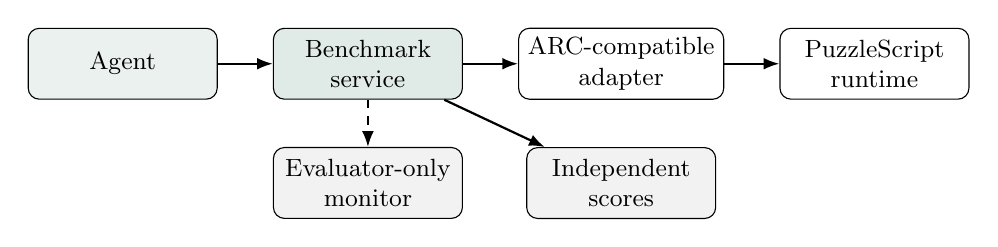
\begin{tikzpicture}[
    node distance=6mm and 7mm,
    box/.style={draw, rounded corners, align=center, minimum height=9mm,
                minimum width=24mm, font=\small},
    arrow/.style={-{Latex[length=2mm]}, thick}
  ]
    \node[box, fill=biugreen!8] (agent) {Agent};
    \node[box, right=of agent, fill=biugreen!12] (bench)
      {Benchmark\\service};
    \node[box, right=of bench] (adapter)
      {ARC-compatible\\adapter};
    \node[box, right=of adapter] (runtime)
      {PuzzleScript\\runtime};
    \node[box, below=of bench, fill=gray!10] (monitor)
      {Evaluator-only\\monitor};
    \node[box, below=of adapter, fill=gray!10] (scores)
      {Independent\\scores};

    \draw[arrow] (agent) -- (bench);
    \draw[arrow] (bench) -- (adapter);
    \draw[arrow] (adapter) -- (runtime);
    \draw[arrow, dashed] (bench) -- (monitor);
    \draw[arrow] (bench) -- (scores);
  \end{tikzpicture}
  \caption{The agent queries the benchmark. The authoritative PuzzleScript
  runtime executes each action once, and the resulting transition updates every
  selected score. Evaluator-only data is exposed through a separate monitor
  credential.}
  \label{fig:architecture}
\end{figure}

The runtime is split because the PuzzleScript engine is distributed as an npm
package. A Node.js service wraps game execution, a Python service adapts it to
the ARC interaction contract, and the benchmark layer adds catalog sampling,
opaque aliases, representation filtering, claims, scoring, persistence, and
monitoring.

\subsection{Independent online scores}

Before an action, the agent may attach a goal-recognition claim and a
rule-inference claim. The environment then executes the action exactly once.
This single transition advances solving progress, labels whether a level was
completed, supplies the target next observation, and updates every enabled
score.

\paragraph{Game solving.}
Let \(c_g\) be the number of completed playable levels and \(m_g\) the total
number of playable levels. The diagnostic completion rate is
\[
  C_g = \frac{c_g}{m_g},
\]
while the primary solving score is binary whole-game completion,
\[
  S_g = \mathbb{I}[c_g=m_g].
\]
If a replay-verified whole-game reference has \(A_g^\star\) actions and the
agent solves the game in \(A_g\) actions, action efficiency is
\[
  E_g=\min\left(1,\frac{A_g^\star}{A_g}\right).
\]
Efficiency is omitted when the agent does not solve the game or a whole-game
reference is unavailable.

\paragraph{Goal recognition.}
Before each action, the agent predicts the probability \(p_t\) that the action
will complete the current level. The real transition supplies label \(y_t\).
The scorecard reports balanced accuracy, F1, coverage, and Brier score,
\[
  \mathrm{Brier}=\frac{1}{T}\sum_{t=1}^{T}(p_t-y_t)^2.
\]
Missing predictions reduce coverage and count as incorrect in the primary
classification denominator.

\paragraph{Rule inference.}
The agent predicts the next integer grid, terminal state, and level delta.
Diagnostics include exact-transition accuracy, exact-frame accuracy, cell
accuracy, changed-cell F1, state accuracy, level-delta accuracy, and coverage.
This tests executable predictive content rather than grading free-form natural
language descriptions of rules.

\subsection{Cross-level transfer}

For target level \(L_k\), the benchmark is intended to provide two matched
conditions:

\begin{itemize}[leftmargin=*]
  \item a \textbf{warm condition} that begins at \(L_1\) and reaches \(L_k\)
        sequentially while the evaluator retains agent memory;
  \item a \textbf{cold condition} initialized directly at \(L_k\), using the
        same game version, representation, and target-level budget.
\end{itemize}

Both conditions are scored independently. If both solve the target level in
\(A_k^{\mathrm{warm}}\) and \(A_k^{\mathrm{cold}}\) actions, a descriptive
relative transfer gain is
\[
  T_k =
  \frac{A_k^{\mathrm{cold}}-A_k^{\mathrm{warm}}}
       {A_k^{\mathrm{cold}}}.
\]
Raw completion and action counts remain primary because this ratio is not
meaningful when either condition fails. Every transfer result will be labeled
\texttt{memory\_reset = user\_managed}; the benchmark cannot prove that an
external agent erased files, caches, or other memory.

\subsection{Reference scope and oracle limitations}

A shortest path under known rules measures execution distance, not optimal rule
learning. An agent that does not know the rules may rationally spend actions on
information gathering, and a globally optimal learning policy is undefined
without a hypothesis space, prior, and exploration-cost objective. Reference
paths therefore support solving-efficiency measurements only. A replay proves
that a path wins in the authoritative engine; unless exactness is separately
established, it does not prove that the path is universally shortest.

\section{Initial Results}

\subsection{Runnable benchmark environment}

The current public manifest identifies benchmark version 0.3.0. The implemented
system provides:

\begin{itemize}[leftmargin=*]
  \item agent-initiated runs over an ARC-compatible REST contract;
  \item deterministic catalog sampling by seed;
  \item separate agent and evaluator-monitor credentials;
  \item optional rendered images, legends, and action semantics;
  \item independent solving, goal-recognition, and rule-inference scorecards;
  \item persisted run envelopes and a browser-based live monitor; and
  \item a deliberatively simple baseline client that exercises the contract.
\end{itemize}

The benchmark does not require an agent URL. The agent calls the environment,
and the monitor observes the run through a separate evaluator credential.

\subsection{Catalog and replay references}

The checked-in public catalog contains 21 games. Every catalog entry has a
replay-verified winning trajectory for its selected first playable level. The
initial bounded breadth-first search attempted 30 sampled first playable levels
and solved 21 within a 60-second or 100,000-state limit. These bounds did not
show that the remaining games were unsolvable.

A later targeted solver generated valid winning paths for the remaining nine
first-level cases. Table~\ref{tab:targeted} reports the replay-verified action
counts. These are valid upper bounds unless separate exactness analysis proves
optimality.

\begin{table}[t]
  \centering
  \small
  \begin{tabular}{lrr}
    \toprule
    Game & Playable level & Winning actions \\
    \midrule
    Fire in Winter      & 2 & 65 \\
    Self Alteration     & 2 & 22 \\
    Collapsing Tiles    & 2 & 14 \\
    Fuse to Green       & 2 & 19 \\
    Dark Pellets        & 3 & 21 \\
    Infected            & 2 & 27 \\
    Extra Push          & 2 & 42 \\
    The Art of Storage  & 2 & 51 \\
    Side Painting       & 3 & 34 \\
    \midrule
    Total               &   & 295 \\
    \bottomrule
  \end{tabular}
  \caption{Replay-verified winning paths for the nine first-level cases that
  exceeded the earlier bounded search. The playable-level number differs from
  the source index when message screens precede a level.}
  \label{tab:targeted}
\end{table}

Together, the search artifacts contain replay-verified first-level winning
trajectories for all 30 sampled games. The current public catalog remains the
checked-in 21-game subset; catalog expansion is part of the research plan.

\subsection{Whole-game reference}

The prototype whole-game solver filters message screens, solves playable levels
sequentially, preserves cumulative progress, and validates the final action
sequence in the original Node.js engine. For
\texttt{ps\_sokoban\_basic-v1}, it replay-verified both playable levels at
action depths 33 and 16, totaling 49 actions. This is currently the only catalog
game with a complete whole-game reference, so action-efficiency results for
other games are intentionally omitted.

\subsection{Measurements not yet available}

\pending{No controlled comparison of frontier agents or baseline agents has
been run on the frozen benchmark suite. The proposal therefore reports no
agent-performance table.}

\pending{The warm/cold transfer endpoints are specified but are not yet
implemented, and no cross-level transfer gain has been measured.}

\pending{No grid-only versus rendered-image versus legend ablation has been
run. The benchmark already records these representation conditions so that the
comparison can be added without changing the score definitions.}

\section{Research Plan}

The remaining work is organized around completing the evaluation substrate and
then running controlled experiments.

\begin{enumerate}[leftmargin=*,label=\textbf{Task \arabic*:}]
  \item \textbf{Complete whole-game references.}
    Enumerate every playable level of each selected game, solve levels
    sequentially, validate every trajectory in the authoritative runtime, and
    distinguish replay-valid paths from references whose shortest-path
    exactness is established.

  \item \textbf{Freeze the benchmark suite and protocol.}
    Select the final game split, budgets, representation conditions, random
    seeds, score aggregation rules, and failure policy. Preserve opaque
    evaluator-controlled game aliases and publish versioned manifests.

  \item \textbf{Run baseline and agent evaluations.}
    Evaluate the trivial client and selected learning agents on one action
    stream per game. Report whole-game completion, level completion, action
    counts, action efficiency where supported, goal-recognition metrics,
    rule-inference metrics, token use, and cost.

  \item \textbf{Implement and evaluate warm/cold transfer.}
    Add matched target-level configurations. The evaluator will run a persistent
    agent in the warm condition and a fresh copy in the cold condition. Report
    target-level completion and action counts first, followed by transfer gain
    only where both conditions solve the level.

  \item \textbf{Analyze kinds of level progression.}
    Annotate whether a later level introduces a new object or mechanic,
    generalizes a known rule, or produces a new interaction among known rules.
    Test whether transfer differs across these categories and inspect negative
    transfer or belief-revision failures.

  \item \textbf{Representation ablations.}
    Compare anonymous integer grids, rendered images, symbolic legends, and
    action semantics under matched games and budgets. Every published result
    will state exactly which representation aids were exposed.

  \item \textbf{Validate robustness and reporting.}
    Check replay determinism, catalog coverage, scorer edge cases, and monitor
    isolation. Publish per-game results and confidence intervals rather than
    collapsing all abilities into one opaque score.
\end{enumerate}

The primary expected outcome is a runnable and reproducible environment for
measuring not only whether an agent completes a PuzzleScript game, but what it
learned about the dynamics and goal, and whether that knowledge improved later
behavior. The main empirical contribution will depend on the completed
whole-game catalog and the controlled agent and transfer studies described
above.

\newpage
\bibliography{proposalbib}
\bibliographystyle{plain}

\end{document}
